\begin{answer}

\begin{figure}[H]
    \centering
    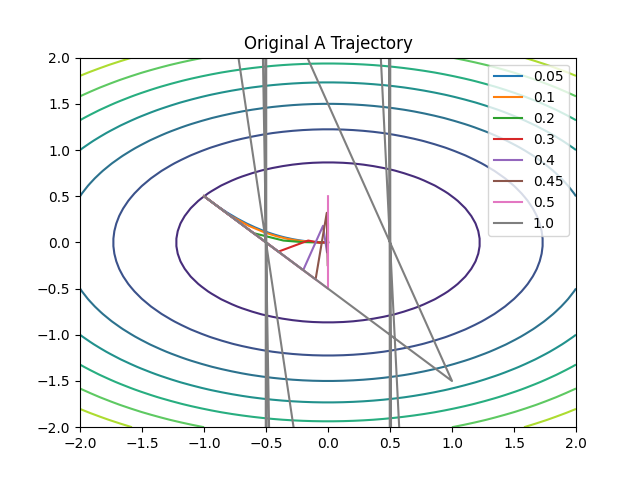
\includegraphics[width=0.5\linewidth]{trajectories.png}
    \caption{trajectories}
    \label{fig:enter-label}
\end{figure}

\begin{figure}[H]
    \centering
    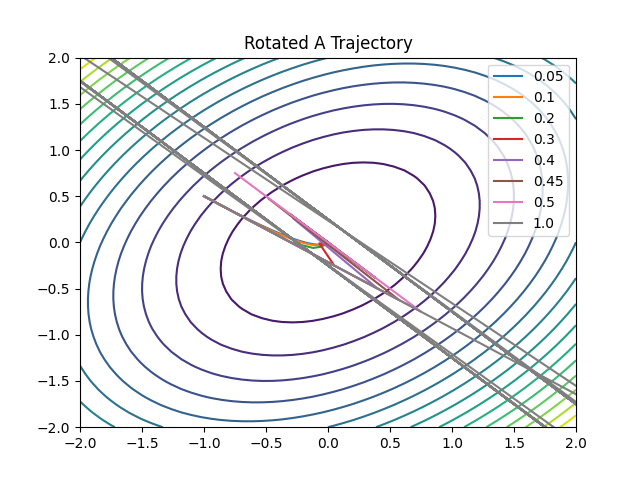
\includegraphics[width=0.5\linewidth]{trajectories_rotated.png}
    \caption{trajectories\_rotated}
    \label{fig:enter-label}
\end{figure}

Discussion:

The experiment results follow our analysis that 1) when $\alpha$ increase, the $T$ first decrease then increase 2) when $\alpha$ is too big, then change in each iteration is significant.

The experiment also shows that the trajectory of converge of rotated $A$ is a rotated version of trajectory of converge of original $A$ 

+++  Output logs as follows +++

[diagonal A, learning rate 0.05] GD took 541 iterations and converged

[diagonal A, learning rate 0.1] GD took 258 iterations and converged

[diagonal A, learning rate 0.2] GD took 115 iterations and converged

[diagonal A, learning rate 0.3] GD took 65 iterations and converged

[diagonal A, learning rate 0.4] GD took 114 iterations and converged

[diagonal A, learning rate 0.45] GD took 257 iterations and converged

[diagonal A, learning rate 0.5] GD took 3 iterations and did not converge

[diagonal A, learning rate 1.0] GD took 23 iterations and did not converge

[rotated A, learning rate 0.05] GD took 531 iterations and converged

[rotated A, learning rate 0.1] GD took 254 iterations and converged

[rotated A, learning rate 0.2] GD took 113 iterations and converged

[rotated A, learning rate 0.3] GD took 64 iterations and converged

[rotated A, learning rate 0.4] GD took 116 iterations and converged

[rotated A, learning rate 0.45] GD took 260 iterations and converged

[rotated A, learning rate 0.5] GD took 3 iterations and did not converge

[rotated A, learning rate 1.0] GD took 22 iterations and did not converge

\end{answer}